\providecommand\NN{{\mathbb N}}
\providecommand\MM{{\mathbb M}}

\section{Background}
In this paper, we use a network architecture called MAMBA, which is centered
around a type of sequence transformation called a state space model(SSM).
\subsection{State Space Models}
State space models take some variable-length sequence of data(text, audio, even
image data), and convert it into some other variable-length sequence of data,
similarly to what a transformer does.
As for how state space models calculate their output sequences, all state space
models are discretizations of the following model, where $x$ is the input
sequence, and $y$ is the output sequence:
$$\begin{aligned}
    n \in \NN \qquad
    A \in \MM^{n \times n} \qquad
    B \in \MM^{n \times 1} \qquad
    C \in \MM^{1 \times n} \\
    \frac{d\vec{s}}{dt} = Bx + A\vec{s}\\
    y = C\vec{s}
\end{aligned}$$
In English, state space models store an internal state that continuously changes
w.r.t the input, and then compute the output at each timestep based on the
internal state.
Intuitively, $\vec{s}$ is the internal state of the model.
For a language model, $\vec{s}$ might store the most recent sentence; For an
image model, it might store nearby lines and shapes.
Notice that this formula uses derivatives, meaning that it only applies to
continuous sequences.

Since we can't store general continuous sequences in hardware, real
implementations of SSMs use discretizations, with some finite timestep.
This means that the actual dynamics of real SSMs are as follows:
$$\begin{aligned}
    \vec{s}_{t+1} &= \exp(\Delta A)\vec{s}_{t} + \Delta B \vec x_{t} \\
    y_{t} &= C \vec{s}_{t+1}
\end{aligned}$$
In addition, real models tend to work with multidimensional sequences, so each
SSM layer is typically a stack of multiple SSMs.

\subsection{hyperparameters}
A common nomenclature for the hyperparameters of state space models is as
follows:
\begin{itemize}
    \item $B$ - The batch size
    \item $L$ - The length of the sequence
    \item $D$ - The number of sequences per instance. This can be thought of as
    the number of "channels" that the layer takes as input.
    \item $N$ - The state size for one SSM
\end{itemize}
To give an example, at any given time step, the total size of the state would be
$BDN$, since we have $B$ instances of SSMs, $D$ separate states vectors within
each SSM, $N$ real number for each state vector.

\subsection{S4}
S4\cite{gu2022efficiently} is one implementation of state space models.
S4 makes all parameters($A$, $B$, $C$, and $\Delta$) fixed within any evaluation
step, and it enforces a special structure on $A$.
Since each parameter is constant with respect to the position in the sequence,
the overall transformation is invariant to translations.
In addition, it can be shown that discrete SSMs are linear transformations of
the input.
This means that SSMs are equivalent to convolutions, and one of the insights of
S4 is that this allows the model to be computed efficiently using fourier
transforms.
In addition, the special structure on $A$ is that it is a normal plus low-rank
(NPLR) matrix. This allows the authors to compute the convolutional kernel much
more efficiently.
Rather than requiring $\tilde O(LN^2)$ time to train as with direct computation,
each S4 "channel" requires only $O(LN + N^2)$ time to train thanks to the
\subsection{Mamba}
Mamba\cite{mamba} adds variable timesteps. This has 2 main consequences.
Firstly, it increases the cost 

\subsection{Background on Formal Language Abilities}
As proven in \cite{ssmformal}, State-Space models are not able 

\subsection{Tests on Formal Language Abilities}
It appears that 

\subsubsection{Formation of "Bad Habits" with Mamba}

% Here is a diagram
% \begin{center}
%     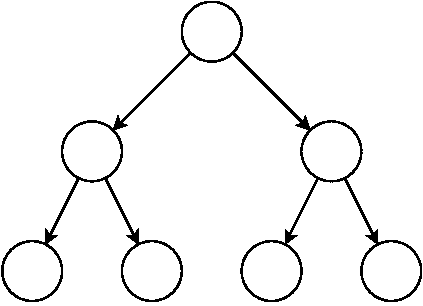
\includegraphics[width=0.5\textwidth]{resources/example-figure.pdf}
% \end{center}